\section{Mean field reinforcement learning methods}

\subsection{Mean field approximation}

\begin{frame}{Mean field approximation}
	The interactions within the population of agents are
	approximated by those between a single agent
	and \alert{the average effect} from the overall population
	or neighboring agents.
	\
	\newline\\
	
	\pause
	\cite[pp.~74--75]{Ising model}\\
	Let's recall the system energy in ising model,
	$$E(s, h)=-\sum_{i}\left(h_{i} s_{i}+\frac{J}{2} \sum_{j \in \mathcal{N}(i)} s_{i} s_{j}\right)$$
	where $\mathcal{N}(i)$ is the set of nearest neighbors of site $i$, $h_i$ is the external field affecting site $i$. The probability is given by $P(s)=\frac{\exp (-E(s, h) / \tau)}{\sum_{s} \exp (-E(s, h) / \tau)}$, where $\tau$ is the system temperature.
	
\end{frame}

\begin{frame}{Mean field approximation}
	$$E(s, h)=-\sum_{i}s_{i}\left(h_{i}+\frac{J}{2} \sum_{j \in \mathcal{N}(i)} s_{j}\right)$$
	we can term $\left(h_{i}+\frac{J}{2} \sum_{j \in \mathcal{N}(i)} s_{j}\right)$ as the equivalent magnetic field $B_i$.\\
	
	Due to thermal fluctuation, we compute the mean value:
	$$\bar{B}_{i}=h_i+\frac{J}{2} \sum_{j} \bar{s}_{j}$$
	If we completely ignore the fluctuations, the average value of the spins of each spin variable is equal $\bar{s}_{j}=\bar{s}$
	then
	$$\bar{B}_{i}=h_i+\frac{z J}{2} \bar{s} \equiv \bar{B}$$
	
	
\end{frame}

\begin{frame}{Mean field approximation}
	The mean field theory provides an approximate solution to $\left\langle s_{i}\right\rangle=\sum_{s} s_{i} P(s)$ through a set of self-consistent mean field
	equations
	$$\left\langle s_{i}\right\rangle=\frac{\exp \left(-\left[h_{i} s_{i}+J \sum_{j \in \mathcal{N}(i)}\left\langle s_{j}\right\rangle\right] / \tau\right)}{1+\exp \left(-\left[h_{i} s_{i}+J \sum_{j \in \mathcal{N}(i)}\left\langle s_{j}\right\rangle\right] / \tau\right)}$$
	which can be solved iteratively by
	$$\left\langle s_{i}\right\rangle ^{(t+1)}=\frac{\exp \left(-\left[h_{i} s_{i}+J \sum_{j \in \mathcal{N}(i)}\left\langle s_{j}\right\rangle ^{(t)}\right] / \tau\right)}{1+\exp \left(-\left[h_{i} s_{i}+J \sum_{j \in \mathcal{N}(i)}\left\langle s_{j}\right\rangle ^{(t)}\right] / \tau\right)}$$
	where $t$ represents the number of iterations.	
\end{frame}

\begin{frame}{Stochastic Game}
	An $N$-agent (or, $N$-player) stochastic game $\Gamma$ is formalized
	by the tuple
	$$\Gamma \triangleq\left(\delta, \mathscr{A}^{1}, \ldots, \mathscr{A}^{N}, r^{1}, \ldots, r^{N}, p, \gamma\right)$$
	
	\pause
	\begin{columns}[c]
		\begin{column}{0.5\textwidth}
			\begin{description} 
				\item[$\delta$] the state space
				\item[$\mathscr{A}^{i}$] the action space of agent $i$
				\item[$r^{i}$] the reward function for agent $i$
				\item[$p$] the transition probability
				\item[$\gamma$] the
				reward discount factor across time
				\item[$s$] an initial state
				\item[$\mathscr{a}$] the joint action
			\end{description}
		\end{column}
	
		\vrule{}
		\begin{column}{0.5\textwidth}
			\begin{itemize}
				\item policy: $\pi^{j}:\delta \mathcal{\rightarrow} Q\left(\mathscr{A}^{j}\right)$, where $\mathscr{A}^{j}$ is the collection of probability distributions over $\mathscr{A}^{j}$.
				\item $\pi \triangleq\left[\pi^{1}, \ldots, \pi^{N}\right]$: the joint policy of all agents, then the value function
				$v_{\pi}^{j}(s)=v^{j}(s ; \pi)=\sum_{t=0}^{\infty} \gamma^{t} \mathbb{E}_{\pi, p}\left[r_{t}^{j} \mid s_{0}=s, \pi\right]$
				\item Q-function: $Q_{\pi}^{j}(s, \boldsymbol{a})=r^{j}(s, \boldsymbol{a})+\gamma \mathbb{E}_{s^{\prime} \sim p}\left[v_{\pi}^{j}\left(s^{\prime}\right)\right]$.
			\end{itemize}
		\end{column}
	\end{columns}
\end{frame}

\begin{frame}{Mean Field MARL}
	As all agents act strategically and evaluate simultaneously their value functions based on the
	joint actions, we factorize the $Q$-function using only the pairwise local interactions:
	$$Q^{j}(s, \boldsymbol{a})=\frac{1}{N^{j}} \sum_{k \in \mathcal{N}(j)} Q^{j}\left(s, a^{j}, a^{k}\right)$$
	where $N^{j}=|\mathcal{N}(j)|$.
	
	\begin{columns}
		\begin{column}{0.4\textwidth}
			\centerline{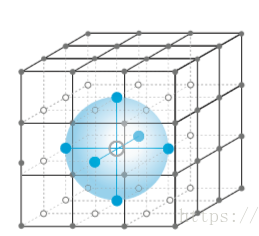
\includegraphics[width = 0.6\textwidth]{Figures/pa.png}}
		\end{column}
		
		\begin{column}{0.6\textwidth}
			\begin{alertblock}{Inference}
				$$Q^{j}\left(\mathbf{s}, \mathbf{a} \right) \approx Q^{j}\left(s, a^{j}, \bar{a}^{j}\right)$$
				where $\bar{a}^{j}=\frac{1}{N^{j}} \sum_{k} a^{k}$.
			\end{alertblock}
		\end{column}
	\end{columns}
\end{frame}

\begin{frame}{Applications in ising model}
	We define the reward for each spin/agent as (to maximize its reward)
	$$r^{j}=h^{j} a^{j}+\frac{J}{2} \sum_{k \in \mathcal{N}(j)} a^{j} a^{k}$$
	To learn an optimal joint policy $\pi^{*}$ for Ising model, we use the stateless $Q$-learning with mean field approximation (MF-$Q$), defined as
	$$Q^{j}\left(a^{j}, \bar{a}^{j}\right) \leftarrow Q^{j}\left(a^{j}, \bar{a}^{j}\right)+\alpha\left[r^{j}-Q^{j}\left(a^{j}, \bar{a}^{j}\right)\right]$$
	\begin{block}{Order parameter}
		$$\xi=\frac{\left|N_{\uparrow}-N_{\downarrow}\right|}{N}$$
		A traditional measure of purity for the Ising model.
	\end{block}
\end{frame}

\begin{frame}{Comparisons with MC}
	\begin{block}{Attention}
		Notice that agents here do not know
		exactly the energy function, but rather use the temporal
		difference learning to approximate $\left\langle a^{j}\right\rangle$ during the learning
		procedure. \nocite{DBLP:journals/corr/abs-1802-05438DBLP:journals/corr/abs-1802-05438}
	\end{block}

	\begin{columns}
		\begin{column}{0.5\textwidth}
			\centerline{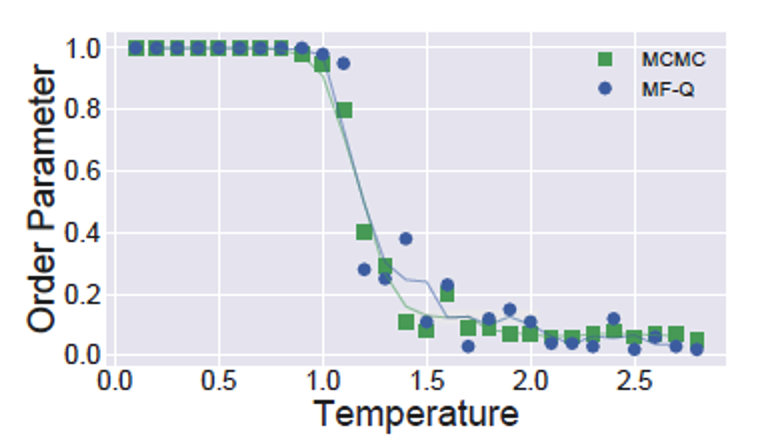
\includegraphics[width = 1.1\textwidth]{Figures/co.png}}
		\end{column}
		\begin{column}{0.5\textwidth}
			This is the first work that manages to solve
			the Ising model via model-free reinforcement learning methods.
		\end{column}
	\end{columns}
	\end{frame}

\begin{frame}{Results}
	\begin{columns}
		\begin{column}{0.7\textwidth}
			\centerline{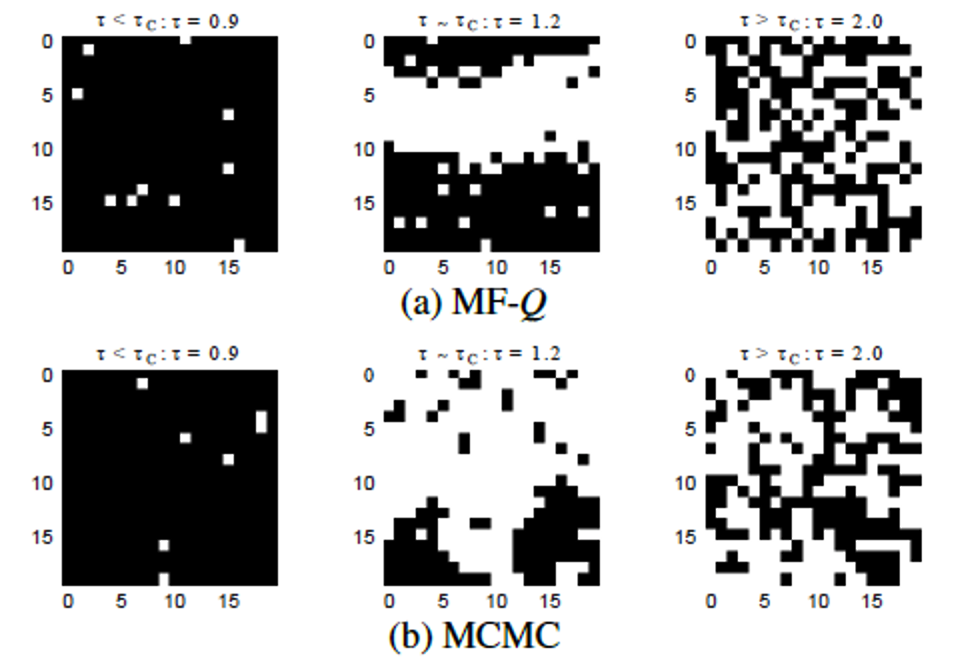
\includegraphics[width = 1.0\textwidth]{Figures/final.png}}
		\end{column}
		\begin{column}{0.3\textwidth}
			\begin{itemize}
				\item As the
				temperature rises ($\tau$ = 1.2, the Curie temperature), some spins become volatile
				and patches start to form as spontaneous magnetization.
			\end{itemize}
		\end{column}
	\end{columns}

	\end{frame}

